\documentclass[10pt]{article}
\usepackage[ngerman]{babel}
\usepackage[utf8]{inputenc}
\usepackage[T1]{fontenc}
\usepackage{amsmath}
\usepackage{amsfonts}
\usepackage{amssymb}
\usepackage[version=4]{mhchem}
\usepackage{stmaryrd}
\usepackage{bbold}
\usepackage{graphicx}
\usepackage[export]{adjustbox}
\graphicspath{ {./images/} }

\begin{document}
\section*{Rechnerarithmetik}
Maschinendarstellbare Zahlen $M$ zur Basis $B$ :

$$
M=\left\{x \in \mathbb{R} \mid x= \pm 0 . m_{1} m_{2} m_{3} \ldots m_{n} \cdot B^{ \pm e_{1} e_{2} \ldots e_{l}}\right\} \cup\{0\}
$$

Dabei gilt $m_{1} \neq 0, m_{i}, e_{i} \in\{0,1, \ldots, B-1\}$ für $i \neq 0$ und $B \in \mathbb{N}(B>1)$

\section*{Der Wert $\widehat{\boldsymbol{\omega}}$ einer solchen Zahl ist definiert als}
$$
\widehat{\omega}=\sum_{i=1}^{n} m_{i} B^{\hat{\mathrm{e}}-i}, \quad \hat{\mathrm{e}}=\sum_{l=1}^{l} e_{i} B^{l-i}
$$

$x$ wird als n -stellige Gleitpunktzahl zur Basis $B$ bezeichnet.\\
Beispiel: $\underbrace{0.3211}_{n=4} \cdot \underbrace{4^{12}}_{l=2}$

\begin{enumerate}
  \item $\hat{e}=1 \cdot 4^{1}+2 \cdot 4^{0}=6$
  \item $\widehat{\omega}=3 \cdot 4^{5}+2 \cdot 4^{4}+1 \cdot 4^{3}+1 \cdot 4^{2}=3664$
\end{enumerate}

\section*{Gleitpunktzahlen}
\begin{itemize}
  \item Single Precision (32 Bit) $\quad V=1$ Bit $\quad E=8$ Bit $\quad M=23$ Bit
  \item Double Precision (64 Bit) $V=1$ Bit $\quad E=11$ Bit $\quad M=52$ Bit
\end{itemize}

Bei allgemeiner Basis $B$ gilt (Maschinengenauigkeit $=e p s$ )

$$
\text { eps }:=\frac{B}{2} \cdot B^{-n}, \quad e p s_{10}:=5 \cdot 10^{-n}
$$

Sie bezeichnet den maximalen relativen Fehler, der durch Rundungen entstehen kann.

$$
\left|\frac{r d(x)-x}{x}\right| \leq 5 \cdot 10^{-n} \quad\left(\text { da } x \geq 10^{e-1}\right)
$$

\section*{Approximations- und Rundungsfehler}
Die Maschinenzahlen sind nicht gleichmässig verteilt. Bei jedem Rechner gibt es eine grösste $\left(x_{\max }\right)$ und kleinste $\left(x_{\min }\right)$ positive Maschinenzahl.

\begin{itemize}
  \item $x_{\text {max }}=B^{e_{\max }}-B^{e_{\max }-n}=\left(1-B^{-n}\right) \cdot B^{e_{\max }}$
  \item $x_{\text {min }}=B^{e_{\text {min }}-1}$
\end{itemize}

\section*{Definition}
Gegeben sei eine Näherung $\tilde{x}$ zu einem exakten Wert $x$

\begin{itemize}
  \item Absoluter Fehler\\
$|\tilde{x}-x|$
  \item Relativer Fehler\\
$\left|\frac{\tilde{x}-x}{x}\right| b z w \cdot \frac{|\tilde{x}-x|}{|x|}$
\end{itemize}

\section*{Fehlerfortpflanzung bei Funktionsauswertungen / Konditionierung}
Näherung für den absoluten und relativen Fehler bei Funktionsauswertungen

$$
\begin{aligned}
\underbrace{|f(\tilde{x})-f(x)|}_{\text {absoluter Fehler von } f(x)} & \approx\left|f^{\prime}(x)\right| \cdot \underbrace{|\tilde{x}-x|}_{\text {absoluter Fehler von } x} \\
\underbrace{\frac{|f(\tilde{x})-f(x)|}{|f(x)|}}_{\text {relativer Fehler von } f(x)} & \approx \underbrace{\frac{\left|f^{\prime}(x)\right| \cdot|x|}{|f(x)|}}_{\text {Konditionszahl } K} . \quad \underbrace{|\tilde{x}-x|}_{\begin{array}{c}
|x| \\
\text { relativer Fehler von } x
\end{array}}
\end{aligned}
$$

Den Faktor $K$ nennt man Konditionszahl.

$$
K:=\frac{\left|f^{\prime}(x)\right| \cdot|x|}{|f(x)|}
$$

Relative Fehlervergrösserung von $x$, bei einer Funktionsauswertung von $f(x)$.

\begin{center}
\begin{tabular}{ll}
- Gut konditionierte Probleme & Konditionszahl ist klein $(\leq 1)$ \\
- Schlecht konditionierte Probleme & Konditionszahl ist gross $(>1)$ \\
\end{tabular}
\end{center}

\section*{Nullstellenprobleme}
Eine Gleichung der Form $F(x)=x$ heisst Fixpunktgleichung.

\begin{itemize}
  \item Ihre Lösungen $\bar{x}$, für die $F(\bar{x})=\bar{x}$ erfüllt ist, heissen Fixpunkte.
\end{itemize}

\section*{Fixpunktiteration}
Gegeben sei $F:[a, b] \rightarrow \mathbb{R}$, mit $x_{0} \in[a, b]$. Die rekursive Folge

$$
x_{x+1} \equiv F\left(x_{n}\right), \quad n=0,1,2, \ldots
$$

Heisst Fixpunktiteration von $F$ zum Startwert $x_{0}$.\\
Sei $F:[a, b] \rightarrow \mathbb{R}$ mit stetiger Ableitung $F^{\prime}$ und $\bar{x} \in[a, b]$ ein Fixpunkt von $F$. Dann gilt für die Fixpunktiteration $x_{n+1}=F\left(x_{n}\right)$

\begin{itemize}
  \item $\quad\left|F^{\prime}(\bar{x})\right|<1 \quad x_{n}$ konvergiert gegen $\bar{x}$, falls $x_{0}$ nahe genug bei $\bar{x}$ liegt anziehend
  \item $\left|F^{\prime}(\bar{x})\right|>1 \quad x_{n}$ konvergiert für keinen Startwert $x_{0} \neq \bar{x}$ abstossend
\end{itemize}

\section*{Banachscher Fixpunktsatz}
Sei $F:[a, b] \rightarrow[a, b]$ und es existiere eine Konstante $\alpha$, wobei gilt

\begin{itemize}
  \item $\alpha(0<\alpha<1)$ : Lipschitz-Konstante
  \item $\forall_{x, y}(x, y \in[a, b])$
\end{itemize}

$$
|F(x)-F(y)| \leq \alpha|x-y|, \quad \frac{|F(x)-F(y)|}{|x-y|} \leq \alpha
$$

Dann gilt

\begin{itemize}
  \item $\quad F$ hat genau einen Fixpunkt $\bar{x}$ in $[a, b]$
  \item Die Fixpunktiteration $x_{n+1}=F\left(x_{n}\right)$ konvergiert gegen $\bar{x}$ für alle Startwerte $x_{0} \in[a, b]$
  \item Es gelten die Fehlerabschätzungen
  \item $\left|x_{n}-\bar{x}\right| \leq \frac{\alpha^{n}}{1-\alpha} \cdot\left|x_{1}-x_{0}\right| \quad$ a-priori Abschätzung
  \item $\left|x_{n}-\bar{x}\right| \leq \frac{\alpha}{1-\alpha} \cdot\left|x_{n}-x_{n-1}\right| \quad$ a-posteriori Abschätzung
\end{itemize}

Berechne die Nullstellen von $p(x)=x^{3}-x+0.3$\\
Fixpunktiteration

$$
x_{n+1}=F\left(x_{n}\right)=x_{n}^{3}+0.3
$$

$F\left(x_{n}\right)$ steigt stetig an\\
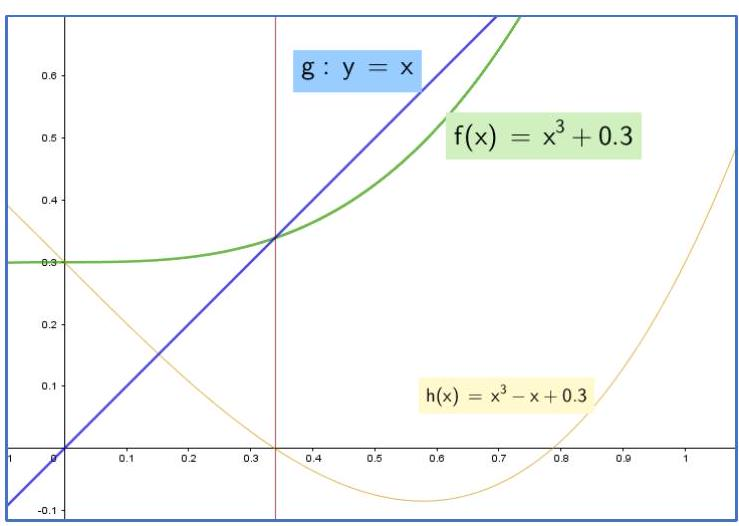
\includegraphics[width=\linewidth]{images/2024_12_29_68ccba06d0091c162fa4g-02}\\
$F: I \rightarrow I$ gilt wenn...

$$
F(a)>a, \quad F(b)<b
$$

Alpha bestimmen / überprüfen

$$
\alpha=\max _{x \in I}\left|F^{\prime}(x)\right| \leq 1
$$

Anzahl Iterationen $n$ berechnen

$$
n \geq \frac{\ln \left(\frac{t o l \cdot(1-\alpha)}{\left|x_{1}-x_{0}\right|}\right)}{\ln \alpha}
$$

\section*{Newton-Verfahren}
Sukzessive Approximation der Funktionskurve $y=f(x)$ durch Tangenten, deren Schnittpunkt mit der x-Achse problemlos berechnet werden kann

Lösung $\xi$ der Gleichung $f(x)=0$ finden.\\
$>$ Startwert $x_{0}$ geeignet wählen (nahe bei $\xi$ )\\
$>$ Iterationsvorschrift:

$$
x_{n+1}=x_{n}-\frac{f\left(x_{n}\right)}{f^{\prime}\left(x_{n}\right)}
$$

Die Folge $\left(x_{n}\right)_{n \in \mathbb{N}}$ konvergiert gegen die Lösung $\xi$ der Gleichung $f(x)=0$.\\
$\left(x_{0}, x_{1}, x_{2}, \ldots\right)$ ist sicher gegeben, wenn im Intervall $[a, b]$, in dem alle Näherungswerte (und die Nullstellen selbst) liegen sollen, die Bedingung

$$
\left|\frac{f(x) \cdot f^{\prime \prime}(x)}{\left[f^{\prime}(x)\right]^{2}}\right|<1
$$

Erfüllt ist (hinreichende Konvergenzbedingung).

\section*{Vereinfachtes Newton-Verfahren}
Statt in jedem Schritt $f^{\prime}\left(x_{n}\right)$ auszurechnen, kann man immer wieder $f^{\prime}\left(x_{0}\right)$ verwenden.

$$
x_{n+1}=x_{n}-\frac{f\left(x_{n}\right)}{f^{\prime}\left(x_{0}\right)}
$$

\section*{Sekantenverfahren}
Der Schnittpunkt von Sekanten durch jeweils zwei Punkte $\left(x_{0}, f\left(x_{0}\right)\right)$ und $\left(x_{1}, f\left(x_{1}\right)\right)$ mit der $x$-Achse, wird berechnet.

$$
x_{n+1}=x_{n}-\frac{x_{n}-x_{n-1}}{f\left(x_{n}\right)-f\left(x_{n-1}\right)} \cdot f\left(x_{n}\right)
$$

\section*{Konvergenzgeschwindigkeit}
Sei $\left(x_{n}\right)$ eine gegen $\bar{x}$ konvergierende Folge. Dann hat das Verfahren die Konvergenzordnung $q \geq 1$ wenn es eine Konstante $c>0$ gibt mit

$$
\left|x_{n+1}-\bar{x}\right| \leq c \cdot\left|x_{n}-\bar{x}\right|^{q}
$$

Für alle $n$.

\begin{itemize}
  \item $q=1 \quad$ lineare Konvergenz $\quad$ verlangt man noch $c<1$.
  \item $q=2$ quadratische Konvergenz
\end{itemize}

\section*{Fehlerabschätzung}
Nullstellensatz von Bolzano\\
Sei $f:[a, b] \rightarrow \mathbb{R}$ stetig mit $f(a) \leq 0 \leq f(b)$ oder $f(a) \geq 0 \geq f(b)$. Dann muss $f$ in $[a, b]$ eine Nullstelle besitzen.

Sei $x_{n}$ also ein iterativ bestimmter Näherungswert einer exakten Nullstelle $\xi$ der stetigen Funktion $F: \mathbb{R} \rightarrow \mathbb{R}$ und es gelte für ein vorgegebene Fehlerschranke / Fehlertolerant $\epsilon>0$

$$
f\left(x_{n}-\epsilon\right) \cdot f\left(x_{n}+\epsilon\right)<0
$$

Dann muss gemäss dem Nullstellensatz im offenen Intervall $\left(x_{n}-\epsilon, x_{n}+\epsilon\right)$ eine Nullstelle $\xi$ liegen und es gilt die Fehlerabschätzung

$$
\left|x_{n}-\xi\right|<\epsilon
$$

Gauss-Algorithmus für ein Gleichungssystem $A x=b$ :

$$
A=\left[\begin{array}{ccc}
a_{11} & \cdots & a_{1 n} \\
\vdots & \ddots & \vdots \\
a_{n 1} & \cdots & a_{n n}
\end{array}\right] \in \mathbb{R}^{n \times n}, \quad x=\left(\begin{array}{c}
x_{1} \\
\vdots \\
x_{n}
\end{array}\right) \in \mathbb{R}^{n}, \quad b=\left(\begin{array}{c}
b_{1} \\
\vdots \\
b_{n}
\end{array}\right) \in \mathbb{R}^{n}
$$

Umformung des Gleichungssystems $A x=b$, in ein äquivalentes Gleichungssystem $\tilde{A} x=b$, so dass die Matrix $\tilde{A}$ als obere Dreiecksmatrix vorliegt.

\begin{itemize}
  \item $\quad z_{j}:=z_{j}-\lambda z_{i} \quad i<j(\lambda \in \mathbb{R}), z_{i}$ ist die $i$-te Zeile des Gleichungssystems
  \item $\quad z_{i} \rightarrow z_{j} \quad$ Vertauschen der $i$-ten und $j$-ten Zeile im System
\end{itemize}

Rekursive Vorschrift für ein Gleichungssystem $\tilde{A} x=b$ :

$$
\begin{gathered}
x_{n}=\frac{b_{n}}{a_{n n}}, x_{n-1}=\frac{b_{n-1}-a_{(n-1) n} \cdot x_{n}}{a_{n-1 n-1}}, \ldots, x_{1}=\frac{b_{1}-a_{12} \cdot x_{2}-\cdots-a_{1 n} \cdot x_{n}}{a_{11}} \\
x_{i}=\frac{b_{i}-\sum_{j=i+1}^{n} a_{i j} \cdot x_{j}}{a_{i i}}, \quad i=n, n-1, \ldots, 1
\end{gathered}
$$

\section*{Fehlerfortpflanzung und Pivotisierung}
Für $i=1, . . n$ :\\
Erzeuge Nullen unterhalb des Diagonalelements in der i-ten Spalte

\begin{itemize}
  \item Suche das betragsgrösste Element unterhalb der Diagonalen in der i-ten Spalte: Wähle $k$ so, dass $\left|a_{k i}\right|=\max \left\{\left|a_{j i}\right| \mid j=i, \ldots n\right\}$
\end{itemize}

$$
\left\{\begin{array}{l}
\text { falls } a_{k i}=0: \quad \text { A ist nicht regulär; stop; } \\
\text { falls } a_{k i} \neq 0: \quad z_{k} \leftrightarrow z_{i}
\end{array}\right.
$$

\begin{itemize}
  \item Eliminationsschritt:
\end{itemize}

Für $j=i+1, \ldots, n$ eliminiere das Element $a_{j i}$ durch

$$
z_{j}:=z_{j}-\frac{a_{j i}}{a_{i i}} \cdot z_{i}
$$

\section*{Determinante}
Gegeben sei eine Matrix $A$, woraus die obere Dreiecksmatrix $\tilde{A}$ entsteht.

\begin{itemize}
  \item $\quad \tilde{a}_{i i}: \quad$ Diagonalelemente von $\tilde{A}$
  \item $\quad l: \quad$ Anzahl Zeilenvertauschungen
\end{itemize}

$$
\operatorname{det}(A)=(-1)^{l} \cdot \operatorname{det}(\tilde{A})=(-1)^{l} \cdot \prod_{i=1}^{n} \tilde{a}_{i i}
$$

Beispiel

$$
\begin{aligned}
\left(\begin{array}{ccc}
3 & 5 & 1 \\
0 & 2 & 2 \\
6 & 14 & 8
\end{array}\right) & =\left(\begin{array}{lll}
3 & 5 & 1 \\
0 & 2 & 2 \\
0 & 4 & 6
\end{array}\right)=\left(\begin{array}{lll}
3 & 5 & 1 \\
0 & 2 & 2 \\
0 & 0 & 2
\end{array}\right) \\
\operatorname{det}(A) & =(3) \cdot(2) \cdot(2)=12
\end{aligned}
$$

Das ursprüngliche Gleichungssystem $\boldsymbol{A} \boldsymbol{x}=\boldsymbol{b}$ lautet mit der $L R$-Zerlegung

$$
L R x=b \Leftrightarrow L y=b \text { und } R x=y
$$

Für eine $n \times n$ Matrix $A$, gibt es $n \times n$ Matrizen $L$ und $R$ mit den Eigenschaften

\begin{itemize}
  \item $L$ ist eine normierte untere Dreiecksmatrix $\operatorname{mit} l_{i i}=1(i=1, \ldots, n)$
  \item $R$ ist eine obere Dreiecksmatrix\\
$\operatorname{mit} r_{i i} \neq 0(i=1, \ldots, n)$
  \item $\quad A=L \cdot R$ ist die $L R$-Zerlegung von $A$.
\end{itemize}

\section*{Zerlegung mit Zeilenvertauschung}
$P_{K}$ erhält man aus der Einheitsmatrix $I_{n}$ durch Vertauschen der $i$-ten und $j$-ten Zeile.\\
Zeilen-Vertauschungen werden durch $P_{1} \ldots P_{n}$ ausgedrückt.

$$
P=\prod_{i=1}^{n} P_{n-i+1}
$$

Mit dieser Permutationsmatrix erhält man dann als $R L-$ Zerlegung

$$
P A=L R
$$

Das lineare Gleichungssystem $A x=b$ lässt sich schreiben als $P A x=P b$ bzw. $L R x=$ $P b$ und in den zwei Schritten lösen

$$
\begin{gathered}
L y=P b \rightarrow y=\cdots \\
R x=y \rightarrow x=\cdots
\end{gathered}
$$

Vertauschung der 1. Und 3. Zeile bei der Matrix

$$
\begin{gathered}
A=\left(\begin{array}{lll}
1 & 2 & 3 \\
4 & 5 & 6 \\
7 & 8 & 9
\end{array}\right) \rightarrow A^{*}=\left(\begin{array}{lll}
7 & 8 & 9 \\
4 & 5 & 6 \\
1 & 2 & 3
\end{array}\right) \\
I^{*} \cdot A=P_{1} \cdot A=A^{*}=\left(\begin{array}{lll}
0 & 0 & 1 \\
0 & 1 & 0 \\
1 & 0 & 0
\end{array}\right)\left(\begin{array}{lll}
1 & 2 & 3 \\
4 & 5 & 6 \\
7 & 8 & 9
\end{array}\right)=\left(\begin{array}{lll}
7 & 8 & 9 \\
4 & 5 & 6 \\
1 & 2 & 3
\end{array}\right) \\
A=\left(\begin{array}{ccc}
-1 & 1 & 1 \\
1 & -3 & -2 \\
5 & 1 & 4
\end{array}\right)=L R \\
i=1, j=2 \rightarrow z_{2}=z_{2}-\frac{1}{(-1)} \cdot z_{1} \rightarrow A_{1}=\left(\begin{array}{ccc}
-1 \\
1-1 & -3+1 & -1+1 \\
5 & 1 & 4
\end{array}\right) \\
i=1, j=3 \rightarrow z_{3}=z_{3}-\underbrace{\frac{5}{(-1)}}_{l_{21}} \cdot z_{1} \rightarrow A_{2}=\left(\begin{array}{ccc}
-1 & 1 & 1 \\
0 & -2 & -1 \\
5-5 & 1+5 & 4+5
\end{array}\right) \\
i=2, j=3 \rightarrow z_{3} \equiv z_{3}-\underbrace{\frac{6}{(-2)}}_{l_{32}} \cdot z_{2} \rightarrow A_{3}=\left(\begin{array}{c}
-1 \\
0 \\
0+0 \\
0
\end{array}\right. \\
R=2
\end{gathered}
$$

Einsetzen in $L$

$$
\begin{gathered}
l_{21}=\frac{1}{-1}=-1, \quad l_{31}=\frac{5}{-1}=-5, \quad l_{32}=\frac{6}{-2}=-3 \\
L=\left(\begin{array}{ccc}
1 & 0 & 0 \\
l_{21} & 1 & 0 \\
l_{31} & l_{32} & 1
\end{array}\right)=\left(\begin{array}{ccc}
1 & 0 & 0 \\
-1 & 1 & 0 \\
5 & -3 & 1
\end{array}\right)
\end{gathered}
$$

Eine Matrix $Q \in \mathbb{R}^{n \times n}$ heisst orthogonal, wenn $Q^{T} \cdot Q=I_{n}$ ist. Dabei ist $I_{n}$ die $n \times n$ Einheitsmatrix.

Sei $A \in \mathbb{R}^{n \times n}$. Eine $Q R$-Zerlegung von $A$ ist eine Darstellung von $A$ als Produkt einer orthogonalen $n \times n$ Matrix $Q$ und einer rechtsoberen $n \times n$ Dreiecksmatrix $R$

$$
A=Q R
$$

Lösung des Gleichungssystems

$$
A x=b \Leftrightarrow Q R x=b \Leftrightarrow R x=Q^{T} b
$$

Algorithmus zur QR-Zerlegung

$$
R:=A, \quad Q:=I_{n}
$$

Für $i=1, \ldots, n-1$ :\\
erzeuge Nullen in $R$ in der $i$-ten Spalte unterhalb der Diagonalen

\begin{enumerate}
  \item $H_{i}$ mit $(n-i+1) \times(n-i+1)$ berechnen
  \item $H_{i}$ mit $I_{i-1}$ Block links oben erweitern $\rightarrow Q_{i}$
  \item $R:=Q_{i} \cdot R$
  \item $Q:=Q \cdot Q_{i}^{T}$
\end{enumerate}

Ablauf

$$
\begin{gathered}
H_{1} \cdot A_{1}=H_{1} \cdot \underbrace{\left(\begin{array}{lll}
* & * & * \\
* & * & * \\
* & * & *
\end{array}\right)}_{A_{1}}=\left(\begin{array}{lll}
* & * & * \\
0 & * & * \\
0 & * & *
\end{array}\right) \rightarrow \underbrace{\left(\begin{array}{cc}
* & * \\
* & *
\end{array}\right)}_{A_{2}} \\
a_{1}=\left(\begin{array}{l}
a_{11} \\
a_{21} \\
a_{31}
\end{array}\right), \quad e_{1}=\left(\begin{array}{l}
1 \\
0 \\
0
\end{array}\right)
\end{gathered}
$$

\begin{enumerate}
  \item $v_{1}:=a_{1}+\operatorname{sign}\left(a_{11}\right) \cdot\left|a_{1}\right| \cdot e_{1}$
  \item $u_{1}:=\frac{1}{\left|v_{1}\right|} \cdot v_{1}$
  \item $H_{1}:=I_{n}-2 u_{1} u_{1}^{T}=Q_{1}$
\end{enumerate}

$$
\begin{gathered}
H_{2} \cdot A_{2}=H_{2} \cdot \underbrace{\left(\begin{array}{ll}
* & * \\
* & *
\end{array}\right)}_{A_{2}}=\left(\begin{array}{ll}
* & * \\
0 & *
\end{array}\right) \\
Q_{2}=\left(\begin{array}{ccc}
1 & 0 & 0 \\
0 & H_{2} & H_{2} \\
0 & H_{2} & H_{2}
\end{array}\right)
\end{gathered}
$$

$$
Q:=Q_{1}^{T} \cdot Q_{2}^{T}, \quad R:=\underbrace{Q_{2} \cdot Q_{1}}_{Q^{-1}} \cdot A
$$

Eine Abbildung $\|\|:. \mathbb{R}^{n} \rightarrow \mathbb{R}$ heisst Vektornorm, wenn die folgenden Bedingungen für alle $x, y \in \mathbb{R}^{n}, \lambda \in \mathbb{R}$ erfüllt sind:

\begin{itemize}
  \item $\|x\| \geq 0$ und $\|x\|=0 \Leftrightarrow x=0$
  \item $\|\lambda x\|=|\lambda| \cdot\|x\|$
  \item $\|x+y\| \leq\|x\|+\|y\|$ "Dreiecksgleichung"
\end{itemize}

Für Vektoren $x=\left(x_{1}, x_{2}, \ldots, x_{n}\right)^{T} \in \mathbb{R}^{n}$ gibt es die folgenden Vektornormen

\begin{itemize}
  \item 1-Norm Summennorm
\end{itemize}

$$
\begin{aligned}
& \|x\|_{1}=\sum_{i=1}^{n}\left|x_{i}\right| \\
& \|x\|_{2}=\sqrt{\sum_{i=1}^{n} x_{i}^{2}} \\
& \|x\|_{\infty}=\max _{i=1, \ldots, n}\left|x_{i}\right|
\end{aligned}
$$

\begin{itemize}
  \item 2-Norm Euklidische Norm
  \item $\infty$-Norm Maximumnorm
\end{itemize}

Für eine $n \times n$ Matrix $A \in \mathbb{R}^{n \times n}$ gibt es die folgenden Matrixnormen

\begin{itemize}
  \item 1-Norm Spaltensummennorm $\|A\|_{1}=\max _{j-1, \ldots, n} \sum_{i=1}^{n}\left|x_{i}\right|$
  \item 2-Norm Spektralnorm $\quad\|A\|_{2}=\sqrt{\rho\left(A^{T} A\right)}$
  \item $\infty$-Norm Zeilensummennorm $\|A\|_{\infty}=\max _{i=1, \ldots, n} \sum_{j=1}^{n}\left|a_{i j}\right|$
\end{itemize}

\section*{Abschätzung für Fehlerhafte Matrizen}
Sei $\|$.$\| eine Norm, A, \tilde{A} \in \mathbb{R}^{n \times n}$ eine reguläre $n \times n$ Matrix und $x, \tilde{x}, b, \tilde{b} \in$ $\mathbb{R}^{n}$ mit $A x=b$ und $\tilde{A} \tilde{x}=\tilde{b}$. Falls

$$
\operatorname{cond}(A) \cdot \frac{\|A-\tilde{A}\|}{\|A\|}<1
$$

Dann gilt

$$
\frac{\|x-\tilde{x}\|}{\|x\|} \leq \frac{\operatorname{cond}(A)}{1-\operatorname{cond}(A) \cdot \frac{\|A-\tilde{A}\|}{\|A\|}} \cdot\left(\frac{\|A-\tilde{A}\|}{\|A\|}+\frac{\|b-\tilde{b}\|}{\|b\|}\right)
$$

\section*{Abschätzung für Fehlerhafte Vektoren}
Sei $\|$. $\|$ eine Norm, $A \in \mathbb{R}^{n \times n}$ eine reguläre $n \times n$ Matrix und $x, \tilde{x}, b, \tilde{b} \in \mathbb{R}^{n}$ mit $A x=b$ und $A \tilde{x}=\tilde{b}$. Dann gilt für den absoluten und den relativen Fehler in $x$ :

\begin{itemize}
  \item $\|x-\tilde{x}\| \leq\left\|A^{-1}\right\| \cdot\|b-\tilde{b}\|$
  \item $\frac{\|x-\tilde{x}\|}{\|x\|} \leq\|A\| \cdot\left\|A^{-1}\right\| \cdot \frac{\|b-\tilde{b}\|}{\|b\|}$, falls $\|b\| \neq 0$\\
$\operatorname{Die}$ Zahl cond $(A)=\|A\| \cdot\left\|A^{-1}\right\|$ nennt man Konditionszahl der Matrix $A$
  \item $\quad \operatorname{cond}(A)$ gross $\rightarrow$ schlechte Konditionierung
\end{itemize}

Untersuchen Sie die Fehlerfortpflanzung im linearen Gleichungssystem $A x=b$ mit

$$
A=\left(\begin{array}{cc}
2 & 4 \\
4 & 8.1
\end{array}\right), \quad b=\binom{1}{1.5}
$$

Für den Fall, dass die rechte Seite von $\tilde{b}$ in jeder Komponente um maximal 0.1 von $b$ abweicht.

$$
\begin{gathered}
\|\tilde{b}-b\|_{\infty} \leq 0.1, \quad\|A\|_{\infty}=\max \{2+4,4+8.1\}=12.1 \\
\left\|A^{-1}\right\|_{\infty}=\left\|\left(\begin{array}{cc}
40.5 & -20 \\
-20 & 10
\end{array}\right)\right\|_{\infty}=60.5 \\
\operatorname{cond}(A)_{\infty}=\|A\|_{\infty} \cdot\left\|A^{-1}\right\|_{\infty}=12.1 \cdot 60.5=732.05 \\
\|x-\tilde{x}\|_{\infty} \leq\left\|A^{-1}\right\|_{\infty} \cdot\|b-\tilde{b}\|_{\infty} \leq 60.5 \cdot 0.1=\underbrace{6.05}_{\text {absoluter Fehler }} \\
\frac{\|x-\tilde{x}\|_{\infty}}{\|x\|_{\infty}} \leq \operatorname{cond}(A)_{\infty} \cdot \frac{\|b-\tilde{b}\|_{\infty}}{\|b\|_{\infty}} \leq 732 \cdot \frac{0.1}{1.5}=\underbrace{48.8}_{\text {relativer Fehler }}
\end{gathered}
$$

Lineare Gleichungssysteme - Fehlerberechnung und Aufwandschätzung

\section*{Aufwandschätzung}
Die Anzahl Gleitkommaoperationen werden in Abhängigkeit von $n$ bestimmt.

$$
\sum_{i=1}^{n} i=\frac{(n+1) \cdot n}{2} \text { und } \sum_{i=1}^{n} i^{2}=\frac{1}{3} n^{3}+\frac{1}{2} n^{2}+\frac{1}{6} n, \quad n=\text { Dimension }
$$

Ein Algorithmus hat die Ordnung $O\left(n^{q}\right)$, wenn $q>0$ die minimale Zahl ist, für die es eine Konstante $C>0$ gibt, so dass der Algorithmus für alle $n \in N$ weniger als

\section*{Beispiel}
Wie viele Gleitkommaoperationen benötigt das Rückwärtseinsetzen gemäss Gauss?

$$
x_{i}=\frac{b_{i}-\sum_{j=i+1}^{n} a_{i j} \cdot x_{j}}{a_{i i}}, \quad i=n, n-1, \ldots, 1
$$

Multiplikation und Division

$$
1+2+3+\cdots+n=\sum_{i=1}^{n} i=\frac{(n+1) \cdot n}{2}
$$

Addition und Subtraktion

$$
0+1+2+\cdots+n-1=\sum_{i=1}^{n-1} i=\frac{(n-1+1) \cdot(n-1)}{2}=\frac{(n-1) \cdot n}{2}
$$

Summe beider Operationstypen

$$
\frac{n^{2}}{2}+\frac{n}{2}+\frac{n^{2}}{2}-\frac{n}{2}=n^{2}
$$

Pascal Isliker

Iterative Verfahren sind effizienter, jedoch kann man keine genauen Lösungen erwarten. Ausgehend von einem Startvektor $x^{(0)}$ berechnet man mittels einer Rechenvorschrift $F: \mathbb{R}^{n} \rightarrow \mathbb{R}^{n}$ iterativ eine Folge von Vektoren

$$
x^{(k+1)}=F\left(x^{(k)}\right) \text { mit } k=0,1,2, \ldots
$$

\section*{Jacobi-Verfahren / Jacobi-Verfahren und Gauss-Seidel-Verfahren}
Zu lösen sei $A x=b$. Die Matrix $A=\left(a_{i j}\right)$ sei zerlegt in der Form $A=L+D+R=$

\section*{Beispiel mit Jacobi}
$$
\begin{gathered}
A x=b, \quad A=\left(\begin{array}{lll}
8 & 5 & 2 \\
5 & 9 & 1 \\
4 & 2 & 7
\end{array}\right), \quad b=\left(\begin{array}{c}
19 \\
5 \\
34
\end{array}\right), \quad x^{(0)}=\left(\begin{array}{c}
1 \\
-1 \\
3
\end{array}\right) \\
x_{1}^{(1)}=\frac{1}{8}\left(19-\sum_{j=1, j \neq 1}^{3} a_{1 j} \cdot x_{j}^{(0)}\right)=\frac{1}{8}(19-(5 \cdot-1+2 \cdot 3))=\frac{18}{8} \\
x_{2}^{(1)}=\frac{1}{9}\left(5-\sum_{j=1, j \neq 2}^{3} a_{2 j} \cdot x_{j}^{(0)}\right)=\frac{1}{9}(5-(5 \cdot 1+1 \cdot 3))=-\frac{1}{3} \\
x_{3}^{(1)}=\frac{1}{7}\left(34-\sum_{j=1, j \neq 3}^{3} a_{3 j} \cdot x_{j}^{(0)}\right)=\frac{1}{7}(34-(4 \cdot 1+2 \cdot-1))=\frac{32}{7}
\end{gathered}
$$

Fixpunktiteration gemäss Jacobi (Gesamtschritt-Verfahren):

$$
\begin{aligned}
& D x^{(k+1)}=-(L+R) x^{(k)}+b \\
& x^{(k+1)}=-D^{-1}(L+R) x^{(k)}+D^{-1} b
\end{aligned}
$$

Implementation /Allgemeine Form gemäss Jacobi

$$
x_{i}^{(k+1)}=\frac{1}{a_{i i}}\left(b_{i}-\sum_{j=1, j \neq i}^{n} a_{i j} \cdot x_{j}^{(k)}\right), \quad i=1, \ldots, n
$$

Fixpunktiteration gemäss Gauss-Seidel (Einzelschritt-Verfahren):

$$
\begin{aligned}
& (D+L) x^{(k+1)}=-R x^{(k)}+b \\
& x^{(k+1)}=-(D+L)^{-1} \cdot R x^{(k)}+(D+L)^{-1} \cdot b
\end{aligned}
$$

Implementation / Allgemeine Form gemäss Gauss-Seidel\\
$x_{i}^{(k+1)}=\frac{1}{a_{i i}}\left(b_{i}-\sum_{j=1}^{i-1} a_{i j} \cdot x_{j}^{(k+1)}-\sum_{j=i+1}^{n} a_{i j} \cdot x_{j}^{(k)}\right), \quad i=1, \ldots, n$

\section*{Lineare Gleichungssysteme - Iterative Verfahren}
Gegeben sei eine Fixpunktiteration

$$
x^{(n+1)}=B x^{(n)}+c=: F\left(x^{(n)}\right)
$$

Für das Gesamtschrittverfahren (Jacobi) gilt

$$
B=-D^{-1}(L+R)
$$

Für das Einzelschrittverfahren (Gauss-Seidel) gilt $\quad B=-(D+L)^{-1} R$

Wobei $B$ eine $n \times n$ Matrix ist und $c \in \mathbb{R}^{n}$. Weiter sei $\|$. $\|$ eine der eingeführten Normen und $\bar{x} \in \mathbb{R}^{n}$ erfülle $\bar{x}=B \bar{x}+c=F(\bar{x})$. Dann heisst

\begin{itemize}
  \item $\bar{x}$ anziehender Fixpunkt, falls $\|B\|<1$
  \item $\bar{x}$ abstossender Fixpunkt, falls $\|B\|>1$
  \item $\left\|x^{(n)}-\bar{x}\right\| \leq \frac{\|B\|^{n}}{1-\|B\|} \cdot\left\|x^{(1)}-x^{(0)}\right\| \quad$ a-priori Abschätzung
  \item $\left\|x^{(n)}-\bar{x}\right\| \leq \frac{\|B\|}{1-\|B\|} \cdot\left\|x^{(n)}-x^{(n-1)}\right\| \quad$ a-posteriori Abschätzung\\
$A$ ist eine diagonaldominante Matrix, falls eines der beiden folgenden Kriterien gilt
  \item $f$ ür alle $i=1, \ldots, n:\left|a_{i i}\right|>\sum_{j=1, j \neq i}^{n}\left|a_{i, j}\right| \quad$ (Zeilensummenkriterium)
  \item für alle $j=1, \ldots, n:\left|a_{j j}\right|>\sum_{i=1, i \neq j}^{n}\left|a_{i, j}\right| \quad$ (Spaltensummenkriterium)
\end{itemize}

Beispiel

$$
A=\left(\begin{array}{ccc}
4 & -1 & 1 \\
-2 & 5 & 1 \\
1 & -2 & 5
\end{array}\right) \rightarrow \sum_{j=1, j \neq i}^{n}\left|a_{i j}\right| \rightarrow\left\{\begin{array}{l}
i=1 \rightarrow 4>2 \\
i=2 \rightarrow 5>3 \\
i=3 \rightarrow 5>3
\end{array}\right.
$$

Fall $A$ diagonaldominant ist, konvergiert das Gesamtschrittverfahren (Jacobi) und auch das Einzelschrittverfahren (Gauss-Seidel) für $A x=b$.

Ein notwendiges und hinreichendes Kriterium für Konvergenz ist\\
Spektralradius $\rho(B)<1$

Die Menge der komplexen Zahlen $\mathbb{C}$ erweitert die Menge der reellen Zahlen $\mathbb{R}$, so dass nun also auch Gleichungen der folgenden Art lösbar werden

$$
x^{2}+1=0
$$

Dafür wird die imaginäre Einheit $i$ mit der folgenden Eigenschaft eingeführt.

$$
i^{2}=-1
$$

Eine komplexe Zahl $z$ ist ein geordnetes Paar $(x, y)$ zweier Zahlen $x$ und $y$.

$$
z=x+i y
$$

Die imaginäre Einheit $i$ ist definiert durch

$$
i^{2}=-1
$$

Die Menge der komplexen Zahlen wird mit $\mathbb{C}$ bezeichnet

$$
\mathbb{C}=\{z \mid z=x+\text { iy mit } x, y \in \mathbb{R}\}
$$

Die reellen Bestandteile $x$ und $y$ von $z$ werden als Real- und Imaginärteil bezeichnet

\begin{itemize}
  \item Realteil von $z \quad \operatorname{Re}(z)=x$
  \item Imaginärteil von $z \quad \operatorname{Im}(z)=y$
\end{itemize}

Die zu $z$ konjugierte komplexe Zahl ist definiert als $z^{*}=x-i y$. Dies entspricht der an der $x$ - Achse gespiegelten Zahl.

Der Betrag einer komplexen Zahl ist definiert als $|z|=\sqrt{x^{2}+y^{2}}=\sqrt{z \cdot z^{*}}$. Dies entspricht der Länge des Zeigers.

\section*{Darstellungsformen}
\begin{itemize}
  \item Normalform $z=x+i y$
  \item Trigonometrische Form $z=r(\cos \varphi+i \cdot \sin \varphi)$
  \item Exponentialform $\quad z=r e^{i \varphi}$
\end{itemize}

$$
\begin{gathered}
x=r \cdot \cos \varphi, \quad y=r \cdot \sin \varphi, \quad r=\sqrt{x^{2}+y^{2}} \\
\varphi=\arcsin \left(\frac{y}{r}\right)=\arccos \left(\frac{x}{r}\right) \\
e^{i \varphi}=\cos \varphi+i \cdot \sin \varphi
\end{gathered}
$$

Beispiel

$$
z=3-11 i
$$

$$
\begin{gathered}
3=r \cdot \cos \varphi, \quad 11=r \cdot \sin \varphi, \quad r=\sqrt{3^{2}+11^{2}}=\sqrt{130} \\
\arcsin \left(\frac{11}{\sqrt{130}}\right)=\varphi=1.3
\end{gathered}
$$

$$
z=\cos (1.3)+i \cdot \sin (1.3), \quad z=\sqrt{130} \cdot e^{i \cdot 1.3}
$$

\begin{center}
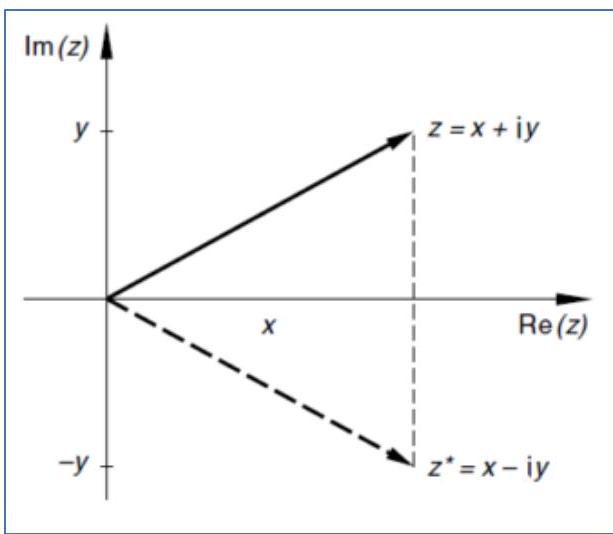
\includegraphics[width=\linewidth]{images/2024_12_29_68ccba06d0091c162fa4g-11}
\end{center}

\section*{Grundrechenarten}
Es sei $z_{1}=x_{1}+i y_{1}$ und $z_{2}=x_{2}+i y_{2}$

\begin{itemize}
  \item Summation $z_{1}+z_{2}=\left(x_{1}+x_{2}\right)+i\left(y_{1}+y_{2}\right)$
  \item Subtraktion $z_{1}-z_{2}=\left(x_{1}-x_{2}\right)+i\left(y_{1}-y_{2}\right)$
\end{itemize}

Multiplikation

$$
\begin{gathered}
z_{1} \cdot z_{2}=\left(x_{1} x_{2}-y_{1} y_{2}\right)+i\left(x_{1} y_{2}+x_{2} y_{1}\right) \\
z_{1} \cdot z_{2}=r_{1} e^{i \varphi_{1}} \cdot r_{2} e^{i \varphi_{2}}=r_{1} r_{2} e^{i\left(\varphi_{1}+\varphi_{2}\right)}
\end{gathered}
$$

Division

$$
\begin{gathered}
\frac{z_{1}}{z_{2}}=\frac{z_{1} \cdot z_{2}^{*}}{z_{2} \cdot z_{2}^{*}}=\frac{\left(x_{1}+i y_{1}\right)\left(x_{2}-i y_{2}\right)}{\left(x_{2}+i y_{2}\right)\left(x_{2}-i y_{2}\right)} \\
=\frac{\left(x_{1} x_{2}+y_{1} y_{2}\right)+i\left(y_{1} x_{2}-x_{1} y_{2}\right)}{x_{2}^{2}+y_{2}^{2}}=\frac{\left(x_{1} x_{2}+y_{1} y_{2}\right)}{x_{2}^{2}+y_{2}^{2}}+i \frac{\left(y_{1} x_{2}-x_{1} y_{2}\right)}{x_{2}^{2}+y_{2}^{2}}
\end{gathered}
$$

$$
\frac{z_{1}}{z_{2}}=\frac{r_{1} e^{i \varphi_{1}}}{r_{2} e^{i \varphi_{2}}}=\frac{r_{1}}{r_{2}} e^{i\left(\varphi_{1}+\varphi_{2}\right)}
$$

\section*{Potenzieren und Radizieren}
Die $n$-te Potenz einer komplexen Zahl lässt sich einfach berechnen, wenn diese in der trigonometrischen oder der Exponentialform vorliegt (Sei $n \in \mathbb{N}$ ):

$$
z=r \cdot e^{i \varphi} \rightarrow z^{n}=\left(r e^{i \varphi}\right)^{n}=r^{n} e^{i n \varphi}=r^{n}(\cos (n \varphi)+i \cdot \sin (n \varphi))
$$

Fundamentalgesetz der Algebra\\
Eine algebraische Gleichung $n$-ten Grades mit komplexen Koeffizienten und Variablen $a_{i}, z \in \mathbb{C}$

$$
a_{n} z^{n}+a_{n-1} z^{n-1}+\cdots+a_{1} z+a_{0}=0
$$

Besitzt in der Menge $\mathbb{C}$ der komplexen Zahlen genau $n$ Lösungen

\section*{Wurzel einer komplexen Zahl}
Eine komplexe Zahl $z$ wird als $n$-te Wurzel von $a \in \mathbb{C}$ bezeichnet, wenn

$$
z^{n}=a \rightarrow z=\sqrt[n]{a}
$$

Lösungen der algebraischen Gleichung $z^{n}=a$

$$
z^{n}=a=r_{0} e^{i \varphi}\left(r_{0}>0 ; n=2,3,4, \ldots\right)
$$

Besitzt in der Menge $\mathbb{C}$ genau $n$ verschiedene Lösungen (Wurzeln)

$$
\begin{gathered}
z_{k}=r\left(\cos \varphi_{k}+i \cdot \sin \varphi_{k}\right)=r e^{i \varphi_{k}} \\
r=\sqrt[n]{r_{0}}, \quad \varphi_{k}=\frac{\varphi+k \cdot 2 \pi}{n}, \quad(f \ddot{u} r k=0,1,2, \ldots, n-1)
\end{gathered}
$$

Die zugehörigen Bildpunkte liegen in der komplexen Zahlenebene auf einem Kreis um den Nullpunkt mit dem Radius $r=\sqrt[n]{r_{0}}$ und bilden die Ecken eines regelmässigen $n$-Ecks.

Es sei $A \in \mathbb{R}^{n \times n} . \lambda \in \mathbb{C}$ heisst Eigenwert von $A$, wenn es einen Vektor $x \in \mathbb{C}^{n} \backslash\{0\}$ gibt mit

$$
A x=\lambda x
$$

$x$ heisst dann Eigenvektor von $A$.

\section*{Eigenschaften von Eigenwerten}
$$
A x-\lambda x=0 \Leftrightarrow\left(A-\lambda I_{n}\right) \cdot x=0
$$

Die Eigenwerte einer Diagonal- oder eine Dreiecksmatrix sind deren Diagonalelemente.

\section*{Polynom und Spur}
Es sei $A \in \mathbb{R}^{n \times n}, \lambda \in \mathbb{C}$. Dann gilt

$$
\lambda \text { ist ein Eigenwert von } A \Leftrightarrow \operatorname{det}\left(A-\lambda I_{n}\right)=0
$$

Die Abbildung $p$ ist definiert durch

$$
p(\lambda) \rightarrow \operatorname{det}\left(A-\lambda I_{n}\right)
$$

Ist ein Polynom vom Grad $n$ und wird charakteristisches Polynom von $A$ genannt. Die Eigenwerte von $A$ sind also die Nullstellen des charakteristischen Polynoms. Damit hat $A$ also genau $n$ Eigenwerte, von denen manche mehrfach vorliegen können.

Die Determinante der Matrix $A$ ist gerade das Produkt ihrer Eigenwerte $\lambda_{1}, \ldots, \lambda_{n}$. Die Summe der Eigenwerte ist gleich der Summe der Diagonalelemente von $A$, d.h. gleich der Spur (tr) von $A$ :

\begin{itemize}
  \item $\operatorname{det}(A)=\lambda_{1} \cdot \lambda_{2} \cdot \ldots \cdot \lambda_{n}$
  \item $\operatorname{tr}(A)=a_{11}+a_{22}+\cdots+a_{n n}=\lambda_{1}+\lambda_{2}+\cdots+\lambda_{n}$
\end{itemize}

Ist $\lambda_{i}$ ein Eigenwert der regulären Matrix $A$, so ist der Kehrwert $\frac{1}{\lambda_{i}}$ ein Eigenwert der inversen Matrix $A^{-1}$.

\section*{Vielfachheit und Spektrum}
Es sei $A \in \mathbb{R}^{n \times n}$. Die Vielfachheit, mit der $\lambda$ als Nullstelle des charakteristischen Polynoms von $A$ auftritt, heisst algebraische Vielfachheit von $\lambda$.

Das Spektrum $\sigma(A)$ ist die Menge aller Eigenwerte von $A$.

\section*{Beispiel}
Berechne Spektrum, Determinante und Spur von

$$
A=\left(\begin{array}{lll}
1 & 0 & 0 \\
2 & 3 & 0 \\
0 & 1 & 2
\end{array}\right)
$$

Eigenwerte

$$
\lambda_{1}=1, \quad \lambda_{2}=3, \quad \lambda_{3}=2
$$

Determinante

$$
\operatorname{det}(A)=\lambda_{1} \cdot \lambda_{2} \cdot \lambda_{3}=6
$$

Spur

$$
\operatorname{tr}(A)=\lambda_{1}+\lambda_{2}+\lambda_{3}=6
$$

Spektrum

$$
\sigma(A)=3
$$

\section*{Eigenschaften von Eigenvektoren}
Seien zwei Eigenvektoren $x, y$ zum selben Eigenwert $\lambda \in \mathbb{C}$ einer Matrix $A \in \mathbb{R}^{n} \times \mathbb{R}^{n}$, so ist $x+y$ und auch jedes Vielfach von $x$ ebenfalls ein Eigenvektor zum Eigenwert $\lambda$ :

$$
\begin{gathered}
A(x+y)=A x+A y=\lambda x+\lambda=\lambda(x+y) \\
A(\mu x)=\mu A x=\mu \lambda x=\lambda \mu x
\end{gathered}
$$

\section*{Eigenraum}
Sei $\lambda \in \mathbb{C}$ ein Eigenwert von $A \in \mathbb{R}^{n \times n}$. Dann bilden die Eigenvektoren zum Eigenwert $\lambda$ zusammen mit dem Nullvektor 0 einen Unterraum von $\mathbb{C}^{n}$, den sogenannten Eigenraum

Der Eigenraum des Eigenwertes $\lambda$ ist die Lösungsmenge des homogenen LGS

$$
\left(A-\lambda I_{n}\right) x=0
$$

Welches nur dann eine nicht-triviale Lösung aufweist, wenn $r g\left(A-\lambda I_{n}\right)<n$.\\
Die Dimension des Eigenraumes von $\lambda$ wird die geometrische Vielfachheit von $\lambda$ genannt. Sie berechnet sich als

$$
n-r g\left(A-\lambda I_{n}\right)
$$

Und gibt die Anzahl der lin. Unabhängigen Eigenvektoren zum Eigenwert $\lambda$.\\
Geometrische und algebraische Vielfachheit eines Eigenwerts müssen nicht gleich sein. Die geom. Vielfachheit ist aber stets kleiner oder gleich der algebraischen Vielfachheit.

Beispiel: Berechne Eigenwerte, Eigenvektoren, Eigenräume

$$
\begin{gathered}
A=\left(\begin{array}{cc}
2 & 5 \\
-1 & -2
\end{array}\right), \quad A-\lambda I_{n}=\left(\begin{array}{cc}
2-\lambda & 5 \\
-1 & -2-\lambda
\end{array}\right) \\
p(\lambda)=\operatorname{det}\left(A-\lambda I_{n}\right)=(2-\lambda)(-2-\lambda)-5 \cdot-1 \\
p(\lambda)=-4+\lambda^{2}+5=\lambda^{2}+1=0 \\
\lambda^{2}=-1=i^{2}
\end{gathered}
$$

Eigenwerte

$$
\lambda_{1}=i, \quad \lambda_{2}=-i
$$

Eigenvektor für $\boldsymbol{\lambda}_{\mathbf{1}}=\boldsymbol{i}$

$$
\begin{gathered}
\left(\begin{array}{cc}
2-i & 5 \\
-1 & -2-i
\end{array}\right) \rightarrow\left(\begin{array}{cc}
2-i & 5 \\
0 & -2-i+\frac{5}{2-i}
\end{array}\right) \\
-2-i+\frac{5}{2-i}=(2-i)(-2-i)+5=1+i^{2}=0 \\
0=(2-i) \cdot x_{1}+5 \cdot x_{2} \\
x_{1}=-\frac{5 x_{2}}{2-i} \cdot \frac{2+i}{2+i}=-\frac{5 \cdot(2+i)}{4-i^{2}}=-\frac{10+5 i}{5}=-2-i \\
x_{1}=\binom{-2-i}{1}
\end{gathered}
$$

Eigenraum

$$
\begin{gathered}
E_{\lambda_{1}}=\left\{x \left\lvert\, x=\mu=\binom{-2-i}{1}\right., \mu \in \mathbb{R}\right\} \\
E_{\lambda_{2}}=\left\{x \left\lvert\, x=\mu=\binom{-2+i}{1}\right., \mu \in \mathbb{R}\right\}
\end{gathered}
$$

\section*{Lineare Gleichungssysteme - Numerische Berechnung von Eigenvektoren und Eigenwerten}
\section*{Ähnliche Matrizen / Diagonalisierbarkeit}
Es seien $A, B \in \mathbb{R}^{n \times n}$ und $T$ eine reguläre Matrix mit ... so heissen $B$ und $A$ zueinander ähnliche Matrizen.

$$
B=T^{-1} A T
$$

Im Spezialfall, dass $B=D$ ein Diagonalmatrix ist, also ... nennt man $A$ diagonalisierbar.

$$
D=T^{-1} A T
$$

\section*{Eigenwerte und Eigenvektoren ähnlicher / diagonalisierbarer Matrizen}
Es seien $A, B \in \mathbb{R}^{n \times n}$ zueinander ähnliche Matrizen. Dann gilt

\begin{enumerate}
  \item $A$ und $B$ haben dieselben Eigenwerte, inkl. deren algebraische Vielfachheit
  \item Ist $x$ ein Eigenvektor zum Eigenwert $\lambda$ von $B$, dann ist $T x$ ein Eigenvektor zum Eigenwert $\lambda$ von $A$.
  \item Falls $A$ diagonalisierbar ist
\end{enumerate}

\begin{itemize}
  \item Diagonalelemente von $D$ sind die Eigenwerte von $A$
  \item Die linear unabhängigen Eigenvektoren von $A$ stehen in den Spalten von $T$
\end{itemize}

Der Spektralradius $p(A)$ einer Matrix $A \in \mathbb{R}^{n \times n}$ ist definiert als

$$
p(A)=\max \left\{|\lambda| \mid \lambda \text { ist ein Eigenwert von } A \in \mathbb{R}^{n \times n}\right\}
$$

Sei $A \in \mathbb{R}^{n \times n}$ eine diagonalisierbare Matrix mit den Eigenwerten $\lambda_{1}, \ldots, \lambda_{n}$ und dem betragsmässig grössten Eigenwert $\lambda_{1}$ mit

$$
\left|\lambda_{1}\right|>\left|\lambda_{2}\right| \geq \cdots \geq\left|\lambda_{n}\right|
$$

\section*{Vektoriteration / von-Mises-Iteration}
So konvergieren für (fast) jeden Startvektor $v^{(0)} \in \mathbb{C}^{n}$ mit Länge 1 die Folgen

$$
v^{(k+1)}=\frac{A v^{(k)}}{\left\|A v^{(k)}\right\|_{2}}, \quad \lambda^{(k+1)}=\frac{\left(v^{(k)}\right)^{T} A v^{(k)}}{\left(v^{(k)}\right)^{T} v^{(k)}}
$$

Für $k \rightarrow \infty$ gegen einen Eigenvektor $v$ zum Eigenwert $\lambda_{1}$ von $A$ (also $v^{(k)} \rightarrow v$ und $\lambda^{(k)} \rightarrow \lambda_{1}$ )

\section*{$Q R$-Verfahren}
Sei $A \in R^{n \times n}$

$$
A_{0}:=A, \quad P_{0}:=I_{n}
$$

Für $i=0,1,2, \ldots$

\begin{itemize}
  \item $A_{i}:=Q_{i} \cdot R_{i}$\\
$Q R$-Zerlegung von $A_{i}$
  \item $A_{i+1}:=R_{i} \cdot Q_{i}$
  \item $P_{i+1}:=P_{i} \cdot Q_{i}$
\end{itemize}

\end{document}